% ============================================================
% HSBI Beamer — ISLP Lecture Series — IMPROVED EDITION
% Chapter 1: Introduction
% ============================================================
\documentclass[aspectratio=169,11pt]{beamer}
\usepackage[utf8]{inputenc}\usepackage[T1]{fontenc}\usepackage[english]{babel}
\usepackage{graphicx}\usepackage{booktabs}\usepackage{amsmath,amssymb,amsfonts}
\usepackage{mathtools}\usepackage{hyperref}\usepackage{xcolor}
\usepackage{verbatim}\usepackage{alltt}
\usepackage{tikz}\usetikzlibrary{calc,arrows.meta,positioning,shapes}
\usepackage{tcolorbox}\tcbuselibrary{skins}

\usetheme{Madrid}\usecolortheme{default}
\setbeamertemplate{navigation symbols}{}
\setbeamertemplate{footline}[frame number]
\setbeamertemplate{blocks}[rounded][shadow=false]
\setbeamertemplate{headline}{%
  \leavevmode\hbox{%
    \begin{beamercolorbox}[wd=\paperwidth,ht=2.2ex,dp=0.9ex]{section in head/foot}%
      {\fontsize{4.6}{5.2}\selectfont%
       \insertsectionnavigationhorizontal{\paperwidth}{}{\hskip0pt plus1filll}}%
    \end{beamercolorbox}}%
}
\setbeamerfont{section in head/foot}{size=\tiny}
\setbeamerfont{palette primary}{size=\tiny}
\setbeamerfont{palette tertiary}{size=\tiny}
\setbeamerfont{section in toc}{size=\footnotesize}

\usepackage{listings}
\definecolor{pyKw}{RGB}{0,0,180}\definecolor{pyStr}{RGB}{20,120,40}
\definecolor{pyCom}{RGB}{120,120,120}\definecolor{accent}{RGB}{38,70,140}
\lstdefinestyle{Pystyle}{language=Python,basicstyle=\ttfamily\footnotesize,
  keywordstyle=\color{pyKw}\bfseries,commentstyle=\color{pyCom}\itshape,
  stringstyle=\color{pyStr},showstringspaces=false,upquote=true,
  columns=fullflexible,breaklines=true,literate={~}{{$\sim$}}1}
\lstset{style=Pystyle}

\AtBeginSection[]{\begin{frame}{Outline}\footnotesize
  \tableofcontents[currentsection,sectionstyle=show/shaded,subsectionstyle=show/show/hide]
\end{frame}}

\newcommand{\islpsource}[1]{%
  \vfill\hfill{\tiny\itshape\color{gray}Source: #1 \textemdash{} ISLP, James et al.\ (2023).}\par
}

\newtcolorbox{takeaway}[1][Takeaway]{enhanced,colback=green!4,colframe=green!50!black,
  boxrule=0pt,leftrule=2.5pt,arc=2pt,fonttitle=\bfseries,title=#1,
  left=2mm,right=2mm,top=1mm,bottom=1mm}
\newtcolorbox{numexample}[1][Worked example]{enhanced,colback=orange!4,colframe=orange!70!black,
  boxrule=0pt,leftrule=2.5pt,arc=2pt,fonttitle=\bfseries,title=#1,
  left=2mm,right=2mm,top=1mm,bottom=1mm}
\newtcolorbox{readme}[1][How to read this]{enhanced,colback=blue!4,colframe=accent,
  boxrule=0pt,leftrule=2.5pt,arc=2pt,fonttitle=\bfseries,title=#1,
  left=2mm,right=2mm,top=1mm,bottom=1mm}

\title{An Introduction to Statistical Learning}
\subtitle{Chapter 1: Introduction \textemdash{} Improved Edition}
\author{Prof.\ Dr.\ Christoph Weisser}\institute{HSBI}
\date{Summer Semester 2026}\graphicspath{{images/}}

\newtcolorbox{exercise}[1][Exercise]{enhanced, fontupper=\footnotesize, colback=purple!4, colframe=purple!55!black, boxrule=0pt, leftrule=2.5pt, arc=2pt, fonttitle=\bfseries, title=#1, left=2mm, right=2mm, top=1mm, bottom=1mm}
\newtcolorbox{solutionbox}[1][Solution]{enhanced, fontupper=\footnotesize, colback=teal!5, colframe=teal!55!black, boxrule=0pt, leftrule=2.5pt, arc=2pt, fonttitle=\bfseries, title=#1, left=2mm, right=2mm, top=1mm, bottom=1mm}

% Reclaim ~2pt of body height (custom nav headline makes full slides tip over by ~1.83pt)
\addtobeamertemplate{frametitle}{}{\vspace{-2pt}}

\newtcolorbox{longexercise}[1][Extended exercise (15 min)]{enhanced, fontupper=\footnotesize, colback=violet!6, colframe=violet!55!black, boxrule=0pt, leftrule=3pt, arc=2pt, fonttitle=\bfseries, title=#1, left=2mm, right=2mm, top=1mm, bottom=1mm}

\newtcolorbox{labnote}[1][Run this live in the lab notebook]{enhanced, fontupper=\footnotesize, colback=cyan!7, colframe=cyan!45!black, boxrule=0pt, leftrule=3pt, arc=2pt, fonttitle=\bfseries, title=#1, left=2mm, right=2mm, top=1mm, bottom=1mm}

\begin{document}
\begin{frame}[plain]\titlepage\end{frame}

\begin{frame}{The course at a glance}
  \footnotesize
  \begin{center}
  \begin{tabular}{@{}c r l@{}}
    & \textbf{Lecture} & \textbf{Topic}\\
    \midrule
    $\blacktriangleright$ & \textbf{1} & \textbf{Ch.\ 1 + 2 --- Introduction; what is statistical learning} \\
     & 2 & Ch.\ 2 --- Accuracy, bias--variance, Bayes classifier, KNN \\
     & 3--4 & Ch.\ 3 --- Linear regression (estimation, inference, diagnostics) \\
     & 5--6 & Ch.\ 4 --- Classification (logistic, LDA/QDA, naive Bayes, ROC) \\
     & 7 & Ch.\ 5 --- Resampling (validation, CV, bootstrap) \\
     & 8 & Ch.\ 6 --- Model selection and regularisation (ridge, lasso) \\
     & 9 & Ch.\ 7 --- Moving beyond linearity (splines, GAMs) \\
     & 10 & Ch.\ 8 --- Tree-based methods (trees, forests, boosting) \\
     & 11 & Ch.\ 10 --- Deep learning (MLPs, CNNs, training) \\
     & 12 & Ch.\ 13 --- Multiple testing (FWER, FDR) \\
  \end{tabular}
  \end{center}
  \vspace{2pt}
  {\scriptsize Twelve sessions of 180 minutes. $\blacktriangleright$ marks today's chapter. Short exercises every $\sim$20 min; extended exercises every $\sim$45 min; each chapter has a companion lab notebook.}
\end{frame}


\begin{frame}{Contents}
  \begin{columns}[t]
    \begin{column}{0.5\textwidth}
      \tableofcontents[hideallsubsections,sections={1-4}]
    \end{column}
    \begin{column}{0.5\textwidth}
      \tableofcontents[hideallsubsections,sections={5-8}]
    \end{column}
  \end{columns}
\end{frame}

\begin{frame}{Notation in this chapter}
  \footnotesize
  \begin{center}
  \begin{tabular}{@{}ll@{}}
    \toprule
    \textbf{Symbol} & \textbf{Meaning} \\
    \midrule
    $n$ & number of observations (sample size) \\
    $p$ & number of variables (predictors) \\
    $x_i$ & predictor value(s) of the $i$-th observation \\
    $y_i$ & response value of the $i$-th observation \\
    $\mathbf{X}$ & $n\times p$ matrix of all predictor values \\
    $x_{ij}$ & value of variable $j$ for observation $i$ \\
    $Y=f(X)+\varepsilon$ & general model: systematic part plus noise \\
    $f$ & unknown true function linking $X$ to $Y$ \\
    $\varepsilon$ & random error term with mean zero \\
    $\hat f$ & estimate of $f$ learned from the data \\
    $\hat Y=\hat f(X)$ & prediction of $Y$ at input $X$ \\
    \bottomrule
  \end{tabular}
  \end{center}
\end{frame}

\begin{frame}{Sources and references}
  \begin{block}{Primary textbook}
    James, G., Witten, D., Hastie, T., Tibshirani, R., \& Taylor, J.\ (2023).
    \emph{An Introduction to Statistical Learning, with Applications in
    Python.} Springer.
  \end{block}
  \begin{block}{About this improved edition}
    Each idea is introduced with motivation, intuition, and a worked
    example. Slide titles are descriptive; key formulas are read
    symbol-by-symbol.
  \end{block}
\end{frame}

\begin{frame}{Learning objectives for this chapter}
  By the end of this chapter you will be able to:
  \begin{itemize}
    \item \textbf{Define} statistical learning and explain why it
          matters.
    \item \textbf{Distinguish} supervised from unsupervised learning,
          and regression from classification.
    \item \textbf{Articulate} the difference between prediction and
          inference, and explain when each goal applies.
    \item \textbf{Read} the standard notation: $n$, $p$, design
          matrix $\mathbf{X}$, response vector $\mathbf{y}$.
    \item \textbf{Recognise} the three motivating data sets (Wage,
          Smarket, NCI60) and the type of question each illustrates.
    \item \textbf{Set up} the Python tooling we will use throughout.
  \end{itemize}
\end{frame}


% ============================================================
\section{Welcome}
% ============================================================

\begin{frame}{Roadmap of this chapter}
  \begin{takeaway}[How this chapter is organised]
    \begin{enumerate}
      \item Why statistical learning matters today.
      \item Definitions: supervised vs.\ unsupervised, regression vs.\
            classification.
      \item Three motivating examples: Wage, Smarket, NCI60.
      \item Notation: $n$, $p$, design matrix $\mathbf{X}$.
      \item The Python ecosystem we will use.
    \end{enumerate}
  \end{takeaway}
  Each section ends with a mini-check question to help you self-assess.
\end{frame}


% ============================================================

\begin{frame}{Why statistical learning is the most-asked-for skill}
  Every discipline now collects more data than it can analyse by hand.
  \begin{takeaway}[The pressure]
    \emph{Storage is essentially free; sensors, transactions, and web
    interactions generate terabytes per minute.} The bottleneck has
    shifted from \emph{collecting} data to \emph{understanding} it.
  \end{takeaway}
  \begin{readme}[Hal Varian quote]
    ``I keep saying that the sexy job in the next ten years will be
    statisticians. And I'm not kidding.''
  \end{readme}
\end{frame}

\begin{frame}{What this course is and is not}
  \begin{columns}[T]
    \begin{column}{0.48\textwidth}
      \begin{block}{What it is}
        A course on the \emph{statistical foundations} of learning.
        We focus on \emph{ideas}, interpretability, and honest
        evaluation.
      \end{block}
    \end{column}
    \begin{column}{0.48\textwidth}
      \begin{alertblock}{What it is not}
        A pure machine-learning engineering course. We will not deploy
        deep nets at production scale.
      \end{alertblock}
    \end{column}
  \end{columns}
  \begin{takeaway}[The course's promise]
    Two questions for every model: (1) \emph{What does this model
    assume about the world?} (2) \emph{What happens when those
    assumptions fail?}
  \end{takeaway}
\end{frame}

\begin{frame}{Prerequisites}
  \begin{block}{Mathematics}
    Linear algebra (matrices, eigenvectors), introductory calculus
    (derivatives, gradients), basic probability.
  \end{block}
  \begin{block}{Statistics}
    Descriptive statistics; simple/multiple linear regression at the
    level of an introductory econometrics course.
  \end{block}
  \begin{block}{Programming}
    Some Python experience is helpful but not required --- we start
    from the basics in the lab sessions.
  \end{block}
\end{frame}

\begin{frame}{The convergence of statistics and computer science}
  \begin{columns}[T]
    \begin{column}{0.48\textwidth}
      \textbf{Statistics emphasises}
      \begin{itemize}
        \item models and assumptions
        \item inference and uncertainty
        \item interpretability
        \item rigorous quantification of error
      \end{itemize}
    \end{column}
    \begin{column}{0.48\textwidth}
      \textbf{Machine learning emphasises}
      \begin{itemize}
        \item algorithms and computation
        \item predictive accuracy
        \item flexibility and scale
        \item large, complex data sets
      \end{itemize}
    \end{column}
  \end{columns}
  \begin{takeaway}[Statistical learning]
    The intersection: methods that are computationally feasible
    \emph{and} statistically principled.
  \end{takeaway}
\end{frame}


% ============================================================
\section{Definitions}
% ============================================================

\begin{frame}{What is statistical learning?}
  \begin{block}{Working definition}
    A vast set of tools for \emph{understanding data}. These tools are
    classified as either \emph{supervised} (we predict an output) or
    \emph{unsupervised} (we look for structure without an output).
  \end{block}
  \begin{readme}
    \begin{itemize}
      \item Supervised: regression (numerical $Y$) and classification
            (categorical $Y$).
      \item Unsupervised: clustering, dimension reduction, density
            estimation.
      \item Closely related fields: machine learning, data mining,
            pattern recognition, predictive analytics.
    \end{itemize}
  \end{readme}
\end{frame}

\begin{frame}{The taxonomy of statistical learning}
  \begin{center}
  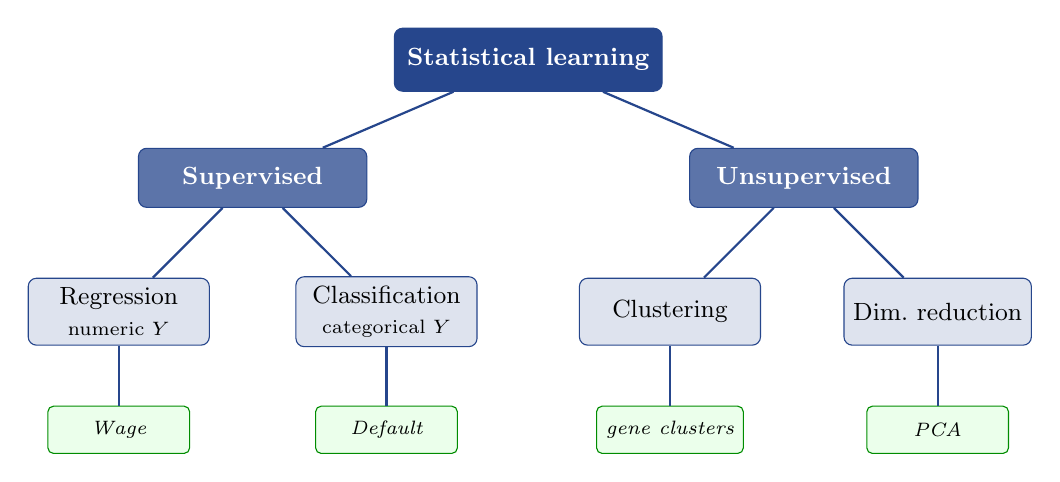
\begin{tikzpicture}[
    root/.style={rounded corners=3pt,draw=accent,fill=accent,text=white,font=\small\bfseries,minimum width=3.4cm,minimum height=0.8cm,align=center},
    branch/.style={rounded corners=3pt,draw=accent,fill=accent!75,text=white,font=\small\bfseries,minimum width=2.9cm,minimum height=0.75cm,align=center},
    leaf/.style={rounded corners=3pt,draw=accent,fill=accent!15,font=\small,minimum width=2.3cm,minimum height=0.85cm,align=center},
    ex/.style={rounded corners=2pt,draw=green!55!black,fill=green!8,font=\scriptsize\itshape,minimum width=1.8cm,minimum height=0.6cm,align=center},
    ed/.style={draw=accent,thick}]
   \node[root]   (r)   at (0,3.2)      {Statistical learning};
   \node[branch] (sup) at (-3.5,1.7)   {Supervised};
   \node[branch] (uns) at (3.5,1.7)    {Unsupervised};
   \node[leaf]   (reg) at (-5.2,0.0)   {Regression\\{\scriptsize numeric $Y$}};
   \node[leaf]   (cla) at (-1.8,0.0)   {Classification\\{\scriptsize categorical $Y$}};
   \node[leaf]   (clu) at (1.8,0.0)    {Clustering};
   \node[leaf]   (dim) at (5.2,0.0)    {Dim.\ reduction};
   \node[ex]     (e1)  at (-5.2,-1.5)  {Wage};
   \node[ex]     (e2)  at (-1.8,-1.5)  {Default};
   \node[ex]     (e3)  at (1.8,-1.5)   {gene clusters};
   \node[ex]     (e4)  at (5.2,-1.5)   {PCA};
   \draw[ed] (r)--(sup); \draw[ed] (r)--(uns);
   \draw[ed] (sup)--(reg); \draw[ed] (sup)--(cla);
   \draw[ed] (uns)--(clu); \draw[ed] (uns)--(dim);
   \draw[ed] (reg)--(e1); \draw[ed] (cla)--(e2);
   \draw[ed] (clu)--(e3); \draw[ed] (dim)--(e4);
  \end{tikzpicture}
  \end{center}
  \begin{takeaway}A response $Y$ splits the field: supervised (predict $Y$) vs.\ unsupervised (discover structure).\end{takeaway}
\end{frame}

\begin{frame}{The fundamental setup}
  We observe a sample
  \[
    \boxed{\;\{(x_1, y_1), (x_2, y_2), \ldots, (x_n, y_n)\}\;}
  \]
  where each $x_i \in \mathbb{R}^p$ is a vector of $p$ \emph{predictors}
  and $y_i$ is a \emph{response}.
  \begin{readme}
    \begin{tabular}{@{}cl@{}}
      \toprule
      \textbf{Symbol} & \textbf{Meaning} \\
      \midrule
      $n$ & Number of observations (sample size) \\
      $p$ & Number of predictors per observation \\
      $x_i$ & Vector of $p$ predictors for observation $i$ \\
      $y_i$ & Response for observation $i$ (number or category) \\
      \bottomrule
    \end{tabular}
  \end{readme}
  In the unsupervised case there is no $y_i$ --- we only have
  $x_1, \ldots, x_n$.
\end{frame}

\begin{frame}{Two distinct goals: prediction vs.\ inference}
  \begin{block}{Prediction}
    Given a new $x_0$, what value of $Y$ should we expect?
  \end{block}
  \begin{block}{Inference}
    How does $Y$ depend on $X$? Which features matter? In what
    direction? By how much?
  \end{block}
  \begin{numexample}[Two examples]
    \emph{Prediction:} given a patient's measurements, will they
    survive 5 years?\\
    \emph{Inference:} which marketing channels actually drive sales?
  \end{numexample}
  \begin{takeaway}[Which goal you have shapes the method]
    Most real problems involve both. Prediction can tolerate a
    black-box model; inference demands an interpretable $\hat f$ whose
    structure we can read off.
  \end{takeaway}
\end{frame}

\begin{frame}{The supervised-learning workflow}
  \begin{center}
  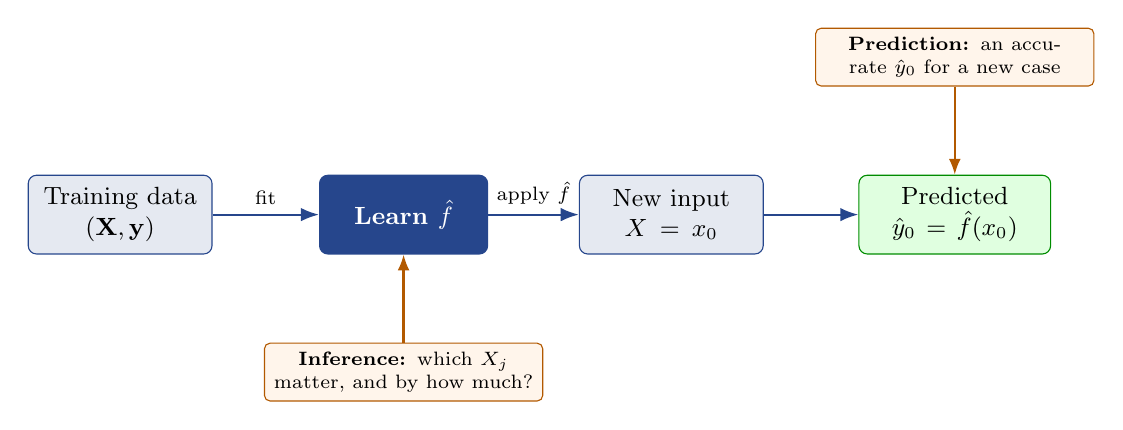
\begin{tikzpicture}[
    stage/.style={rounded corners=3pt,draw=accent,fill=accent!12,align=center,font=\small,text width=2.1cm,minimum height=1.0cm},
    model/.style={rounded corners=3pt,draw=accent,fill=accent,text=white,align=center,font=\small\bfseries,text width=1.9cm,minimum height=1.0cm},
    outbox/.style={rounded corners=3pt,draw=green!55!black,fill=green!12,align=center,font=\small,text width=2.2cm,minimum height=1.0cm},
    note/.style={rounded corners=2pt,draw=orange!70!black,fill=orange!8,align=center,font=\scriptsize,text width=3.3cm},
    arr/.style={-{Latex[length=2.3mm]},thick,draw=accent},
    narr/.style={-{Latex[length=2mm]},thick,draw=orange!70!black}]
   \node[stage]  (train) at (0,0)    {Training data\\$(\mathbf{X},\mathbf{y})$};
   \node[model]  (fit)   at (3.6,0)  {Learn $\hat f$};
   \node[stage]  (newx)  at (7.0,0)  {New input\\$X=x_0$};
   \node[outbox] (pred)  at (10.6,0) {Predicted\\$\hat y_0=\hat f(x_0)$};
   \draw[arr] (train)--(fit)  node[midway,above,font=\scriptsize]{fit};
   \draw[arr] (fit)--(newx)   node[midway,above,font=\scriptsize]{apply $\hat f$};
   \draw[arr] (newx)--(pred);
   \node[note] (inf) at (3.6,-2.0)  {\textbf{Inference:} which $X_j$ matter, and by how much?};
   \draw[narr] (inf)--(fit);
   \node[note] (prd) at (10.6,2.0)  {\textbf{Prediction:} an accurate $\hat y_0$ for a new case};
   \draw[narr] (prd)--(pred);
  \end{tikzpicture}
  \end{center}
  \begin{takeaway}We learn $\hat f$ from training data, then reuse it on new inputs --- prediction targets $\hat y_0$; inference targets the structure of $\hat f$.\end{takeaway}
\end{frame}


\begin{frame}{Exercise 1.1 --- Prediction vs.\ Inference [Concept]}
\begin{exercise}
For each scenario, decide whether the \emph{primary} goal is
\textbf{prediction} or \textbf{inference}, and justify in one line.
\begin{enumerate}
  \item A bank wants to know \emph{which} applicant characteristics
        raise default risk, and \emph{by how much}.
  \item A streaming service auto-fills the rating a user would give a
        film they have not seen.
  \item An economist estimates the effect of a minimum-wage rise on
        employment.
  \item A hospital flags high-risk patients from lab values; it need
        not explain the reasoning.
  \item For a \emph{pure inference} goal, would you prefer a linear
        model or a deep neural network? Why?
\end{enumerate}
\end{exercise}
\end{frame}

\begin{frame}{Solution --- Exercise 1.1 (1/2)}
\begin{solutionbox}
\textbf{How to decide.} Ask what the \emph{deliverable} is: an accurate
value $\hat Y$ for new cases means \emph{prediction}; a statement about
\emph{how} $Y$ depends on the $X_j$ (which ones, in which direction, by
how much) means \emph{inference}.
\begin{enumerate}
  \item \textbf{Inference.} The deliverable is which predictors matter
        and the direction/magnitude of their effect, not a single
        forecast. The give-away words are ``\emph{which}
        characteristics'' and ``\emph{by how much}'' --- both ask about
        the structure of $f$, so the bank needs a model whose
        coefficients it can read off and defend.
  \item \textbf{Prediction.} Only the accuracy of the filled-in rating
        matters; \emph{why} the user would rate it that way is
        irrelevant. The rating is consumed directly by the recommender
        --- nobody inspects the mechanism --- so a black-box $\hat f$
        is perfectly acceptable.
  \item \textbf{Inference.} The goal is a causal effect size (a
        coefficient with a confidence interval). A forecast of
        employment alone would not answer the policy question ``what
        happens \emph{if} the minimum wage rises?''.
\end{enumerate}
\end{solutionbox}
\end{frame}

\begin{frame}{Solution --- Exercise 1.1 (2/2)}
\begin{solutionbox}
\begin{enumerate}\setcounter{enumi}{3}
  \item \textbf{Prediction.} Accurate flagging is what counts;
        interpretability is secondary here. The hospital acts on the
        flag itself (direct attention to high-risk patients), so the
        model is judged purely on its held-out accuracy.
  \item \textbf{Linear model.} Its coefficients have direct meaning
        and come with standard errors, confidence intervals and
        $p$-values, so we can quantify \emph{how} $Y$ depends on each
        $X_j$. A deep network predicts well but is a black box --- its
        weights do not answer an inference question.
\end{enumerate}
\textbf{Rule of thumb:} prediction cares only about $\hat Y$;
inference cares about the \emph{structure} of $f$.

\smallskip
{\itshape Common mistake: classifying by the \emph{tool} instead of the
\emph{question} (``it uses regression, so it must be inference'').
Any model can serve either goal --- what decides is whether the answer
you hand over is $\hat Y$ itself or the shape of $f$.}
\end{solutionbox}
\end{frame}


% ============================================================
\section{Examples}
% ============================================================

\begin{frame}{Three motivating examples set the tone}
  We will study three very different data sets, each illustrating one
  major flavour of problem.
  \begin{takeaway}
    \begin{itemize}
      \item \textbf{Wage}: regression, mostly inference.
      \item \textbf{Smarket}: classification, weak signal.
      \item \textbf{NCI60}: unsupervised, structure discovery.
    \end{itemize}
  \end{takeaway}
\end{frame}

\begin{frame}{Example 1: Wage --- a regression problem}
  \begin{block}{The data}
    Survey of 3{,}000 men working in the central Atlantic region of
    the U.S. Response \texttt{wage} is continuous, so this is a
    \emph{regression} problem.
  \end{block}
  \begin{readme}[Variables]
    \begin{itemize}
      \item Response: \texttt{wage} (annual income in thousands of
            dollars).
      \item Predictors: \texttt{age}, \texttt{year},
            \texttt{education}, plus marital status, race, region.
    \end{itemize}
  \end{readme}
\end{frame}

\begin{frame}{Wage data: wage vs.\ age, year, and education}
  \begin{center}
    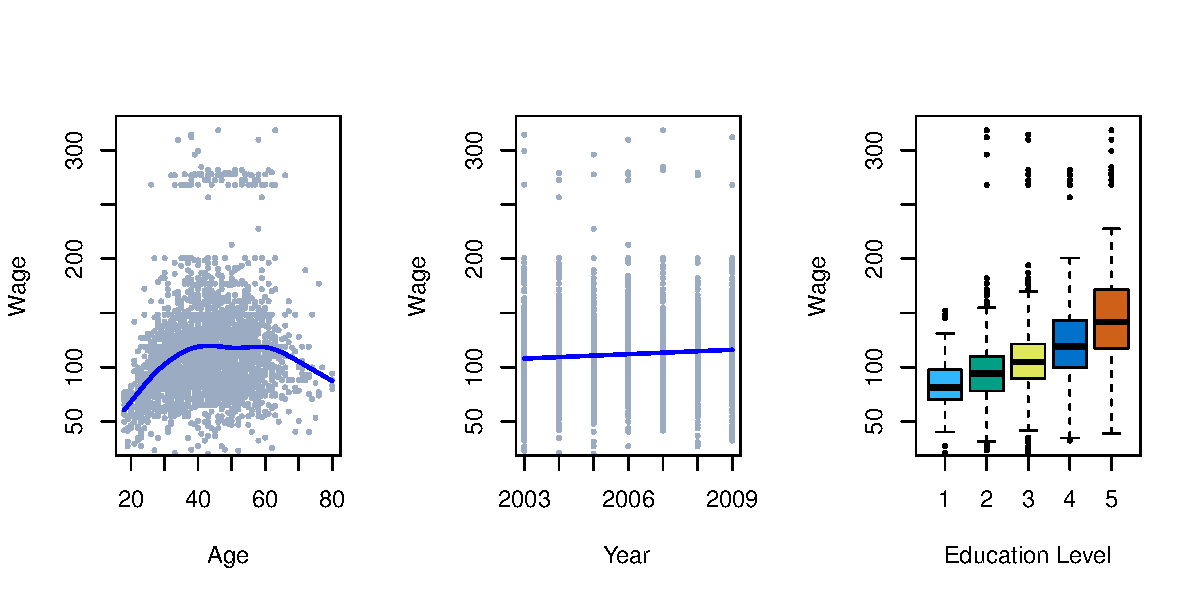
\includegraphics[width=0.95\textwidth,height=0.66\textheight,keepaspectratio]{1_1.pdf}
  \end{center}
  \islpsource{Figure 1.1}
\end{frame}

\begin{frame}{What the Wage plots tell us}
  Reading the three panels left to right:
  \begin{itemize}
    \item \textbf{Wage vs.\ age}: increasing until around 60, then a
          slight decline --- a \emph{nonlinear} relationship.
    \item \textbf{Wage vs.\ year}: a slow upward trend --- wages grow
          modestly over time.
    \item \textbf{Wage vs.\ education}: a strong, monotone effect ---
          higher education levels mean higher wages.
  \end{itemize}
  \begin{takeaway}[Modelling implication]
    A purely linear regression in \texttt{age} would miss the
    curvature. We will need polynomial terms or splines (Ch.~7).
  \end{takeaway}
\end{frame}

\begin{frame}{Wage data up close: age, year, and education}
  \begin{center}
    
\includegraphics[width=0.98\textwidth,height=0.58\textheight,keepaspectratio]{ch01_wage_overview.png}
  \end{center}
  \begin{takeaway}Wage rises then dips with age (nonlinear), drifts gently upward over the years (linear), and climbs steeply with education.\end{takeaway}
\end{frame}

\begin{frame}{Example 2: Smarket --- a classification problem}
  \begin{block}{The data}
    Daily percentage returns of the S\&P~500 from 2001--2005. Response
    \texttt{Direction} (\texttt{Up}/\texttt{Down}) is binary, so this
    is a \emph{classification} problem.
  \end{block}
  \begin{readme}[Variables]
    \begin{itemize}
      \item Response: \texttt{Direction} (\texttt{Up} / \texttt{Down}).
      \item Predictors: \texttt{Lag1}, \ldots, \texttt{Lag5} (previous
            five days' returns) and \texttt{Volume}.
    \end{itemize}
  \end{readme}
\end{frame}

\begin{frame}{Smarket: previous-day returns by direction}
  \begin{center}
    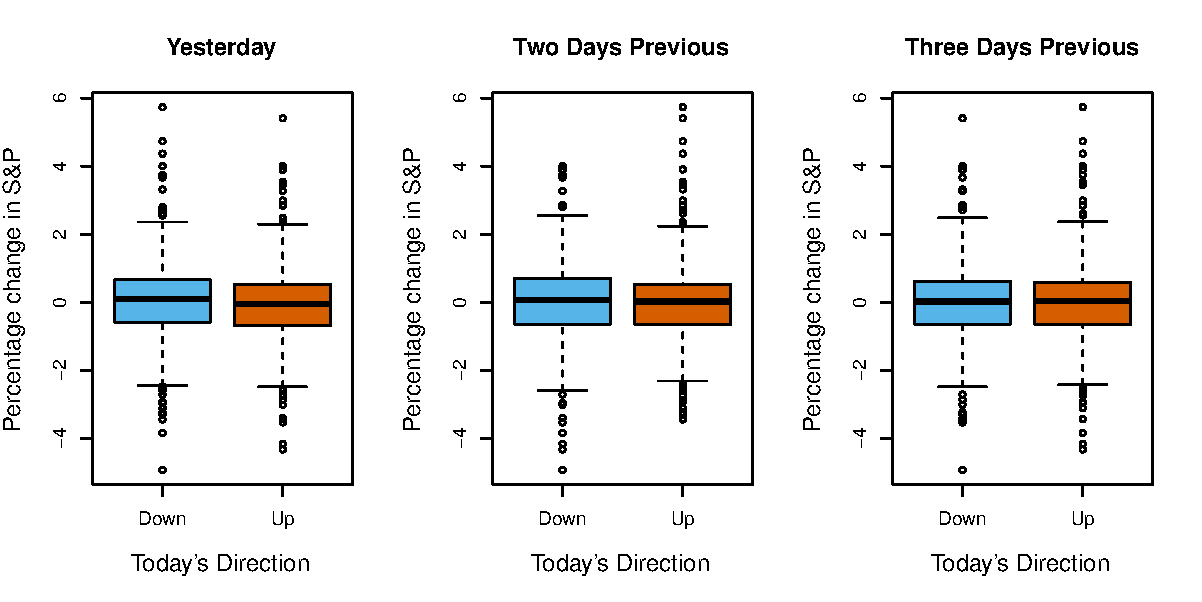
\includegraphics[width=0.92\textwidth,height=0.66\textheight,keepaspectratio]{1_2.pdf}
  \end{center}
  \islpsource{Figure 1.2}
\end{frame}

\begin{frame}{Reading the boxplots}
  Each panel compares yesterday's, two days ago, and three days ago
  returns for days where the market went \texttt{Up} vs.\
  \texttt{Down}.
  \begin{alertblock}{The bad news}
    The boxplots are \emph{nearly identical}. Past returns barely
    predict the next day's direction --- consistent with the
    efficient-markets hypothesis.
  \end{alertblock}
  \begin{takeaway}[A cautionary tale]
    Even when a problem ``looks like'' a classification problem, it
    does not follow that we can solve it well. Prediction is only
    possible if predictors actually carry information about the
    response.
  \end{takeaway}
\end{frame}

\begin{frame}{Recreating Figure 1.2 from the raw Smarket data}
  \begin{center}
\includegraphics[width=0.88\textwidth,height=0.5\textheight,keepaspectratio]{ch01_x_smarket_lag_boxplots.png}\end{center}
  \begin{takeaway}Median \texttt{Lag1} from \texttt{Smarket.csv}: $+0.10\,\%$ before Down days vs.\ $-0.05\,\%$ before Up days --- a $0.15$-point gap against boxes spanning $\pm 0.6\,\%$. Yesterday's return barely separates the classes: market prediction is hard.\end{takeaway}
\end{frame}

\begin{frame}{Smarket: a tiny but real signal}
  \begin{center}
    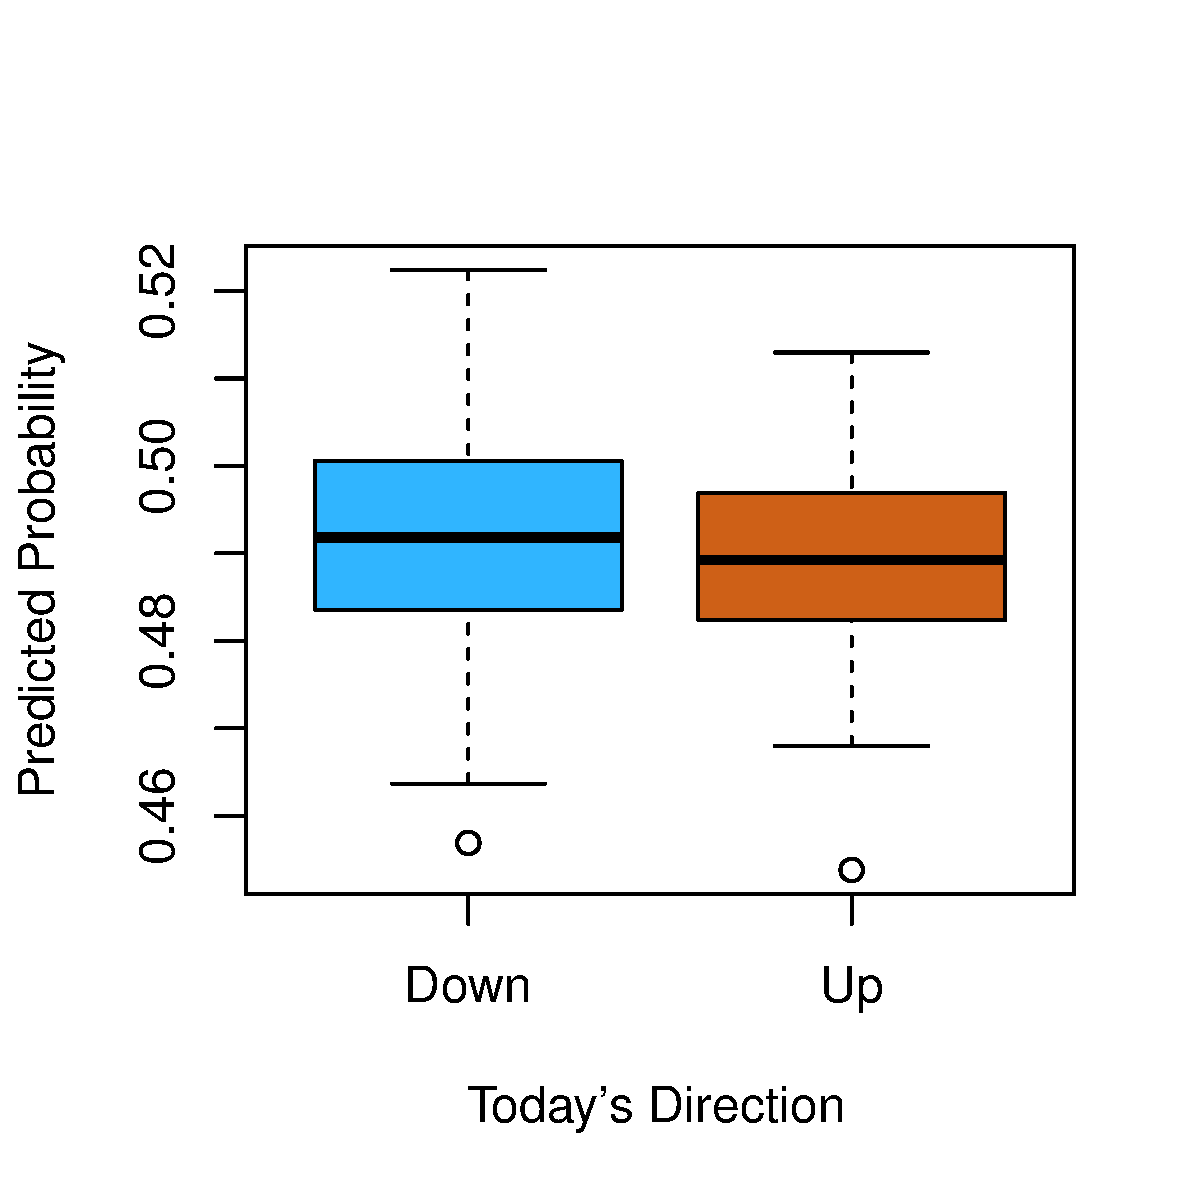
\includegraphics[width=0.78\textwidth,height=0.62\textheight,keepaspectratio]{1_3.pdf}
  \end{center}
  Quadratic discriminant analysis on the same predictors yields about
  $60\,\%$ accuracy on held-out 2005 data --- a small but potentially
  profitable edge.
  \islpsource{Figure 1.3}
\end{frame}

\begin{frame}{Example 3: NCI60 --- an unsupervised problem}
  \begin{block}{The data}
    NCI60: 64 cancer cell lines, 6{,}830 gene expression measurements
    each. \emph{No} response variable --- we don't know what to predict.
  \end{block}
  \begin{takeaway}
    Goal: discover \emph{groups} of similar cell lines (clustering)
    and \emph{visualise} the high-dimensional data in 2D (dimension
    reduction). This is unsupervised learning.
  \end{takeaway}
\end{frame}

\begin{frame}{NCI60: the first two principal components}
  \begin{center}
    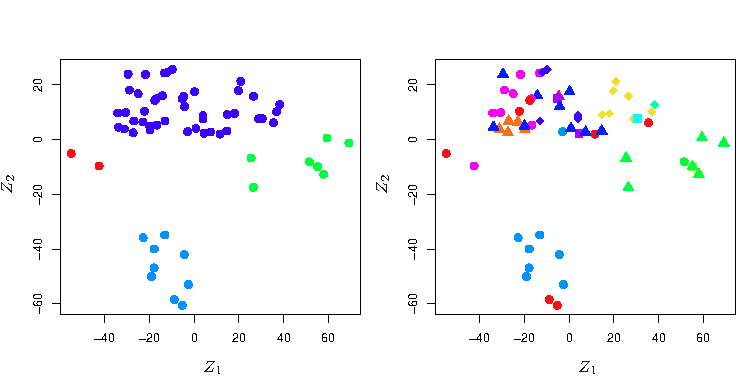
\includegraphics[width=0.78\textwidth,height=0.66\textheight,keepaspectratio]{1_4.pdf}
  \end{center}
  Cell lines of the same cancer type cluster together. PCA recovered
  biologically meaningful structure from raw gene expression alone
  --- without ever seeing the labels.
  \islpsource{Figure 1.4}
\end{frame}

\begin{frame}{What the three examples illustrate}
  \begin{takeaway}[The course's three flavours]
    \begin{itemize}
      \item \textbf{Wage}: a quantitative response, mostly an
            \emph{inference} question $\to$ regression.
      \item \textbf{Smarket}: a categorical response, mostly a
            \emph{prediction} question $\to$ classification.
      \item \textbf{NCI60}: no response, structural questions $\to$
            unsupervised learning.
    \end{itemize}
  \end{takeaway}
  These three flavours structure the rest of the course.
\end{frame}


% ============================================================
\begin{frame}{Mini-check: types of problems}
  \begin{readme}[Quick self-assessment]
    For each of the following, decide: regression, classification, or
    unsupervised?
    \begin{enumerate}
      \item Predicting next year's GDP growth from macro indicators.
      \item Detecting which customers will cancel their subscription.
      \item Grouping news articles into topics without prior labels.
      \item Forecasting house prices from features.
      \item Identifying the digit shown in a 28$\times$28 pixel image.
    \end{enumerate}
  \end{readme}
  \begin{takeaway}[Answers]
    1.\ regression. 2.\ classification. 3.\ unsupervised. 4.\ regression.
    5.\ classification.
  \end{takeaway}
\end{frame}



\begin{frame}{Notation: $n$, $p$, and the design matrix}
  \begin{block}{Sample size and dimension}
    \begin{itemize}
      \item $n$: number of observations
      \item $p$: number of predictors (features)
    \end{itemize}
  \end{block}
  \begin{readme}[Generic notation]
    \begin{tabular}{@{}cl@{}}
      \toprule
      \textbf{Object} & \textbf{Notation} \\
      \midrule
      Scalars & lower-case italic, $a, b, x, y$ \\
      Vectors of length $n$ & bold lower-case, $\mathbf{a}$ \\
      Vectors of length $\ne n$ \& matrices & bold upper-case, $\mathbf{A}, \mathbf{X}$ \\
      \bottomrule
    \end{tabular}
  \end{readme}
\end{frame}

\begin{frame}{The design matrix}
  Stack the predictor vectors as rows:
  \[
    \boxed{\;
      \mathbf{X} =
      \begin{pmatrix}
        x_{11} & x_{12} & \cdots & x_{1p} \\
        x_{21} & x_{22} & \cdots & x_{2p} \\
        \vdots & \vdots & \ddots & \vdots \\
        x_{n1} & x_{n2} & \cdots & x_{np}
      \end{pmatrix} \in \mathbb{R}^{n\times p}.
    \;}
  \]
  \begin{readme}
    \begin{itemize}
      \item Row $i$: vector $x_i = (x_{i1}, \ldots, x_{ip})^\top$ ---
            one observation, all predictors.
      \item Column $j$: vector $\mathbf{x}_j$ --- all observations, one
            predictor.
      \item $x_{ij}$: value of the $j$-th predictor for the $i$-th
            observation.
    \end{itemize}
  \end{readme}
\end{frame}

\begin{frame}{Anatomy of the data: the matrix $\mathbf{X}$ and the vector $\mathbf{y}$}
  \begin{center}
  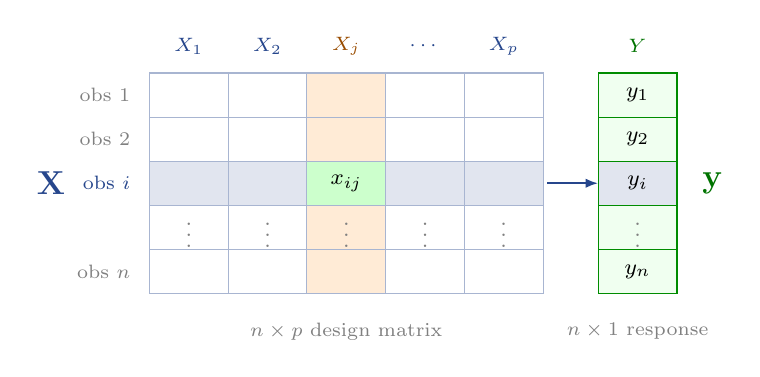
\begin{tikzpicture}[
    cell/.style={draw=accent!40,minimum width=1.0cm,minimum height=0.56cm,font=\footnotesize,inner sep=0pt},
    col/.style={font=\scriptsize\bfseries,text=accent},
    yc/.style={draw=green!55!black,minimum width=1.0cm,minimum height=0.56cm,font=\footnotesize,inner sep=0pt,fill=green!6}]
    \node[col] at (0,0.62){$X_1$}; \node[col] at (1.0,0.62){$X_2$};
    \node[col,text=orange!60!black] at (2.0,0.62){$X_j$}; \node[col] at (3.0,0.62){$\cdots$};
    \node[col] at (4.0,0.62){$X_p$};
    \foreach \ry in {0,1,2,3,4}{
      \pgfmathsetmacro\yy{-\ry*0.56}
      \foreach \cx in {0,1,2,3,4}{
        \pgfmathsetmacro\xx{\cx*1.0}
        \ifnum\ry=2
          \ifnum\cx=2 \node[cell,fill=green!20] at (\xx,\yy){$x_{ij}$};
          \else \node[cell,fill=accent!14] at (\xx,\yy){}; \fi
        \else\ifnum\ry=3
          \ifnum\cx=2 \node[cell,fill=orange!16,text=gray] at (\xx,\yy){$\vdots$};
          \else \node[cell,text=gray] at (\xx,\yy){$\vdots$}; \fi
        \else
          \ifnum\cx=2 \node[cell,fill=orange!16] at (\xx,\yy){};
          \else \node[cell] at (\xx,\yy){}; \fi
        \fi\fi
      }
      \ifnum\ry=0 \node[left,font=\scriptsize,text=gray] at (-0.62,\yy){obs 1};\fi
      \ifnum\ry=1 \node[left,font=\scriptsize,text=gray] at (-0.62,\yy){obs 2};\fi
      \ifnum\ry=2 \node[left,font=\scriptsize,text=accent] at (-0.62,\yy){obs $i$};\fi
      \ifnum\ry=4 \node[left,font=\scriptsize,text=gray] at (-0.62,\yy){obs $n$};\fi
    }
    \node[font=\large\bfseries,text=accent] at (-1.75,-1.12){$\mathbf{X}$};
    \node[font=\scriptsize,text=gray] at (2.0,-3.0){$n\times p$ design matrix};
    \begin{scope}[shift={(5.7,0)}]
      \node[col,text=green!45!black] at (0,0.62){$Y$};
      \node[yc] at (0,0){$y_1$}; \node[yc] at (0,-0.56){$y_2$};
      \node[yc,fill=accent!14] at (0,-1.12){$y_i$};
      \node[yc,text=gray] at (0,-1.68){$\vdots$}; \node[yc] at (0,-2.24){$y_n$};
      \node[font=\large\bfseries,text=green!45!black] at (0.95,-1.12){$\mathbf{y}$};
      \node[font=\scriptsize,text=gray] at (0,-3.0){$n\times 1$ response};
    \end{scope}
    \draw[-{Latex[length=1.6mm]},accent,thick] (4.55,-1.12)--(5.2,-1.12);
  \end{tikzpicture}
  \end{center}
  \begin{takeaway}A \textbf{row} is one observation $x_i$ (all predictors); a \textbf{column} is one predictor across all observations; $x_{ij}$ sits at row $i$, column $j$. Supervised learning pairs each row of $\mathbf X$ with its response $y_i$.\end{takeaway}
\end{frame}

\begin{frame}{The response and estimates}
  \begin{block}{Response vector}
    \[ \mathbf{y} = (y_1, y_2, \ldots, y_n)^\top \in \mathbb{R}^n. \]
  \end{block}
  \begin{readme}[The hat convention]
    Estimated quantities wear a hat: $\hat{\beta}, \hat{f}, \hat{y}$.
    The hat reminds us that these are computed from a sample and
    therefore have sampling variability.
  \end{readme}
  \begin{numexample}[Common usage]
    Predicted (fitted) values: $\hat{y}_i$.\\
    Residuals: $e_i = y_i - \hat{y}_i$.\\
    Train vs.\ test: subscripts $\mathrm{tr}$ and $\mathrm{te}$.
  \end{numexample}
\end{frame}


\begin{frame}{Exercise 1.2 --- Regression, Classification, or Unsupervised? [Concept]}
\begin{exercise}
Classify each task. If it is \emph{supervised}, also say whether it is
\textbf{regression} or \textbf{classification} and name the response
$Y$.
\begin{enumerate}
  \item Predict a used car's selling price from mileage, age, brand.
  \item Segment 64 cell lines described by 6{,}830 gene-expression
        values into similar groups.
  \item Predict whether an incoming e-mail is spam.
  \item Forecast tomorrow's electricity demand (MWh) from weather and
        calendar features.
  \item Reduce 20 survey questions to a few underlying ``factors''.
  \item Recognise which of the digits 0--9 a handwritten image shows.
\end{enumerate}
\end{exercise}
\end{frame}

\begin{frame}{Solution --- Exercise 1.2 (1/2)}
\begin{solutionbox}
\textbf{Method.} First look for a designated response $Y$: none
$\Rightarrow$ \emph{unsupervised}. If there is one, its \emph{type}
decides: quantitative $\Rightarrow$ regression, qualitative
$\Rightarrow$ classification.
\begin{enumerate}
  \item \textbf{Supervised regression}; $Y=$ price (quantitative).
        Past sales provide labelled pairs (features, price), and the
        target is a number on a continuous scale --- exactly the
        setting squared-error loss is made for.
  \item \textbf{Unsupervised} (clustering); there is no response $Y$.
        All $6{,}830$ gene-expression values are inputs --- none of
        them is a label --- and the goal is to \emph{discover} groups,
        not to predict anything.
  \item \textbf{Supervised classification}; $Y=$ spam / not-spam
        (binary, qualitative). The training e-mails are already
        labelled, and the output is a category, not a quantity.
\end{enumerate}
\end{solutionbox}
\end{frame}

\begin{frame}{Solution --- Exercise 1.2 (2/2)}
\begin{solutionbox}
\begin{enumerate}\setcounter{enumi}{3}
  \item \textbf{Supervised regression}; $Y=$ demand in MWh
        (quantitative). Weather and calendar variables are the
        predictors; historical demand records supply the labels.
  \item \textbf{Unsupervised} (dimension reduction); no response $Y$.
        We seek a few latent ``factors'' that summarise 20 correlated
        answers --- PCA / factor-analysis territory (Ch.~12).
  \item \textbf{Supervised classification}; $Y=$ digit $0,\ldots,9$
        (10 qualitative classes). The pixel intensities are
        \emph{numeric predictors}, but numeric inputs do not make it a
        regression --- the output is one of ten categories, and a
        ``7'' is not numerically closer to an ``8'' than to a ``1'' in
        any sense that squared error could use.
\end{enumerate}
\textbf{Decision rule:} no $Y$ $\Rightarrow$ unsupervised. With a $Y$:
quantitative $\Rightarrow$ regression, qualitative $\Rightarrow$
classification. The type of the \emph{response} decides --- not the
predictors.

\smallskip
{\itshape Common mistake: letting the predictors vote --- e.g.\ calling
digit recognition ``regression'' because pixels are numbers, or task 1
``classification'' because \texttt{brand} is categorical. Only the
type of $Y$ matters.}
\end{solutionbox}
\end{frame}


% ============================================================
\section{Tools}
% ============================================================

\begin{frame}{Why Python?}
  Python is the most widely used language in industry data science
  and machine learning.
  \begin{block}{The scientific stack}
    NumPy, pandas, matplotlib, scikit-learn, statsmodels, ISLP. All
    free, mature, and well-documented.
  \end{block}
  \begin{readme}
    The \emph{first} edition of the textbook used R. The methods are
    identical --- only the syntax changes. We will use Python
    throughout.
  \end{readme}
\end{frame}

\begin{frame}{The core scientific stack}
  \begin{tabular}{ll}
    \toprule
    \textbf{Library} & \textbf{Role} \\
    \midrule
    \texttt{numpy} & numerical arrays, linear algebra \\
    \texttt{pandas} & data frames, CSV I/O, group-by \\
    \texttt{matplotlib} & plotting (low-level) \\
    \texttt{seaborn} & plotting (statistical) \\
    \texttt{scipy} & scientific routines (optimisation, stats) \\
    \texttt{statsmodels} & inference-oriented regression / GLM \\
    \texttt{scikit-learn} & general-purpose ML \\
    \texttt{ISLP} & book companion package \\
    \bottomrule
  \end{tabular}
\end{frame}

\begin{frame}[fragile]{Standard imports}
  \begin{lstlisting}
import numpy as np                 # arrays and linear algebra
import pandas as pd                # data frames (tables)
import matplotlib.pyplot as plt    # plotting

# models, data splitting / CV, and error metrics:
from sklearn.linear_model    import LinearRegression, LogisticRegression
from sklearn.model_selection import train_test_split, cross_val_score
from sklearn.metrics         import mean_squared_error, accuracy_score

from ISLP import load_data         # the book's datasets
  \end{lstlisting}
  Adopt these as the default first cell of every notebook.
\end{frame}

\begin{frame}[fragile]{30-second tour: NumPy}
  \begin{lstlisting}
import numpy as np
x = np.array([1, 2, 3, 4])      # 1-D array (a vector)
A = np.array([[1, 2], [3, 4]])  # 2-D array (a matrix)

x.shape       # (4,)   -- one axis of length 4
A.shape       # (2, 2) -- 2 rows, 2 columns
A @ A         # matrix product
np.linalg.inv(A)                # matrix inverse
np.mean(x), np.std(x)           # mean and standard deviation
  \end{lstlisting}
\end{frame}

\begin{frame}[fragile]{30-second tour: pandas}
  \begin{lstlisting}
import pandas as pd
df = pd.read_csv("Wage.csv")    # load CSV into a DataFrame

df.shape           # (3000, 11) -- 3000 rows, 11 columns
df.head()          # show the first 5 rows
df["wage"].mean()  # mean of a single column
df.groupby("education")["wage"].mean()  # mean wage per group
df.describe()      # summary statistics for every column
  \end{lstlisting}
\end{frame}

\begin{frame}[fragile]{30-second tour: scikit-learn}
  \begin{lstlisting}
from sklearn.linear_model import LinearRegression

X = df[["age", "year"]].values  # predictor matrix (n x 2)
y = df["wage"].values           # response vector (n,)
model = LinearRegression()      # choose the model...
model.fit(X, y)                 # ...and estimate it from data

print(model.coef_, model.intercept_)  # fitted slopes, intercept
yhat = model.predict(X)         # predicted wage for each row
  \end{lstlisting}
  Every scikit-learn model follows the same \texttt{fit / predict}
  API.
\end{frame}


% ============================================================
\section{Datasets}
% ============================================================

\begin{frame}{Datasets used throughout the book}
  ISLP comes with a curated collection of datasets that illustrate
  every major method.
  \begin{takeaway}
    All accessible via the \texttt{ISLP} Python package, also as CSV
    files. Most are tabular and modest in size --- chosen to run on a
    laptop in seconds.
  \end{takeaway}
\end{frame}

\begin{frame}{Datasets at a glance (1/2)}
  \footnotesize
  \begin{tabular}{lrrll}
    \toprule
    \textbf{Name} & $n$ & $p$ & \textbf{Response} & \textbf{Used in} \\
    \midrule
    Wage         & 3000 &  10 & wage (num.)        & Ch.~1, 7 \\
    Smarket      & 1250 &   8 & Direction (binary) & Ch.~1, 4 \\
    NCI60        &   64 & 6830 & --- (unsup.)       & Ch.~1, 12 \\
    Auto         &  392 &   8 & mpg (num.)         & Ch.~3 \\
    Boston       &  506 &  12 & medv (num.)        & Ch.~3, 8 \\
    Carseats     &  400 &  10 & Sales (num.)       & Ch.~3, 8 \\
    Credit       &  400 &  10 & Balance (num.)     & Ch.~3, 6 \\
    Default      & 10000 &  3 & default (binary)   & Ch.~4 \\
    Heart        &  303 &  13 & AHD (binary)       & Ch.~4, 8 \\
    \bottomrule
  \end{tabular}
\end{frame}

\begin{frame}{Datasets at a glance (2/2)}
  \footnotesize
  \begin{tabular}{lrrll}
    \toprule
    \textbf{Name} & $n$ & $p$ & \textbf{Response} & \textbf{Used in} \\
    \midrule
    Caravan      & 5822 &  85 & Purchase (binary)  & Ch.~4 \\
    OJ           & 1070 &  17 & Purchase (binary)  & Ch.~8, 9 \\
    Hitters      &  322 &  19 & Salary (num.)      & Ch.~6, 8 \\
    College      &  777 &  17 & Apps (num.)        & Ch.~6 \\
    BrainCancer  &   88 &   8 & survival           & Ch.~11 \\
    USArrests    &   50 &   4 & --- (unsup.)       & Ch.~12 \\
    Bikeshare    & 8645 &  14 & bikers (num.)      & Ch.~4 \\
    \bottomrule
  \end{tabular}
\end{frame}


\begin{frame}{Exercise 1.3 --- Notation: $n$, $p$, and $\mathbf{X}$ [Math]}
\begin{exercise}
For five patients we record \texttt{age} (yrs), \texttt{BMI}, and
resting heart rate \texttt{HR}; the response is systolic blood
pressure \texttt{SBP}.
\begin{center}\vspace{-2mm}\footnotesize
\begin{tabular}{cccc|c}
\toprule
Patient & age & BMI & HR & SBP \\
\midrule
1 & 45 & 24.0 & 70 & 128 \\
2 & 60 & 29.5 & 82 & 145 \\
3 & 52 & 26.1 & 75 & 138 \\
4 & 38 & 22.3 & 68 & 120 \\
5 & 71 & 31.0 & 90 & 158 \\
\bottomrule
\end{tabular}
\end{center}\vspace{-3mm}
\begin{enumerate}\setlength\itemsep{0pt}
  \item State $n$ and $p$.
  \item Give the dimensions of the design matrix $\mathbf{X}$ and the
        response vector $\mathbf{y}$.
  \item Write the predictor vector $x_3$ and give the value $x_{2,3}$.
  \item If an intercept column of ones is added, what are the
        dimensions of the model matrix?
  \item Is this a regression or a classification problem?
\end{enumerate}
\end{exercise}
\end{frame}

\begin{frame}{Solution --- Exercise 1.3 (1/2)}
\begin{solutionbox}
\begin{enumerate}
  \item Count the rows and the predictor columns of the table:
        $n = 5$ observations (one per patient); $p = 3$ predictors
        (\texttt{age}, \texttt{BMI}, \texttt{HR}). \texttt{SBP} is the
        response, \emph{not} a predictor --- the variable we model is
        never counted in $p$.
  \item Rows $=$ patients, columns $=$ predictors, so
        $\mathbf{X}\in\mathbb{R}^{5\times 3}$; stacking the five
        responses gives
        $\mathbf{y}=(128,\,145,\,138,\,120,\,158)^\top
        \in\mathbb{R}^{5}$ (a $5\times1$ column).
  \item Read off \emph{row} 3 of the table:
        $x_3 = (52,\ 26.1,\ 75)^\top$ --- all predictors of patient 3.
        For $x_{2,3}$ the \emph{first} index is the row (observation),
        the \emph{second} the column (predictor): predictor $3$
        (\texttt{HR}) of patient $2$, i.e.\ $x_{2,3}=82$.
\end{enumerate}
\end{solutionbox}
\end{frame}

\begin{frame}{Solution --- Exercise 1.3 (2/2)}
\begin{solutionbox}
\begin{enumerate}\setcounter{enumi}{3}
  \item Adding a column of ones gives
        $\tilde{\mathbf{X}}\in\mathbb{R}^{5\times 4}$: the row count
        stays at $n=5$, while the column count grows from $p=3$ to
        $p+1=4$ --- the extra column of ones multiplies the intercept
        $\beta_0$ in a linear model.
  \item \textbf{Regression}: \texttt{SBP} is quantitative (blood
        pressure in mmHg, on a continuous scale), so regression
        methods and squared-error loss apply.
\end{enumerate}
\textbf{Note on indexing:} $x_{ij}$ is row $i$ (observation),
column $j$ (predictor). Row $i$ is one patient across all predictors;
column $j$ is one predictor across all patients.

\smallskip
{\itshape Common mistake: reading $x_{2,3}$ column-first as ``column 2,
row 3'', which would give the \texttt{BMI} of patient 3 ($26.1$)
instead of the correct $x_{2,3}=82$; and counting the response
\texttt{SBP} into $p$, which would wrongly give $p=4$.}
\end{solutionbox}
\end{frame}


% ============================================================
\section{Roadmap}
% ============================================================

\begin{frame}{The book in one slide}
  \begin{tabular}{rl}
    \toprule
    Ch.\,2  & Statistical Learning (foundations) \\
    Ch.\,3  & Linear Regression \\
    Ch.\,4  & Classification (logistic, LDA, QDA, naive Bayes) \\
    Ch.\,5  & Resampling Methods (CV, bootstrap) \\
    Ch.\,6  & Linear Model Selection and Regularisation \\
    Ch.\,7  & Moving Beyond Linearity (splines, GAMs) \\
    Ch.\,8  & Tree-Based Methods (CART, RF, boosting, BART) \\
    Ch.\,9  & Support Vector Machines \\
    Ch.\,10 & Deep Learning \\
    Ch.\,11 & Survival Analysis and Censored Data \\
    Ch.\,12 & Unsupervised Learning (PCA, clustering) \\
    Ch.\,13 & Multiple Testing \\
    \bottomrule
  \end{tabular}
\end{frame}

\begin{frame}{The narrative arc}
  \begin{itemize}
    \item Chapters 2--4 establish the \emph{vocabulary} and
          \emph{baseline} methods (regression and classification).
    \item Chapter 5 teaches you how to \emph{honestly evaluate}
          models.
    \item Chapter 6 takes the linear model beyond OLS (subset
          selection, ridge, lasso).
    \item Chapters 7--10 add increasing flexibility: nonlinear, trees,
          SVMs, deep nets.
    \item Chapter 11 specialises to time-to-event data.
    \item Chapter 12 returns to unsupervised problems.
    \item Chapter 13 reasons about many simultaneous tests.
  \end{itemize}
  \begin{takeaway}The arc: build \emph{vocabulary} and baseline methods, learn to \emph{evaluate honestly}, then add \emph{flexibility} step by step before specialising.\end{takeaway}
\end{frame}


% ------------------------------------------------------------
% Extended (integrative) exercise --- end of Roadmap section
% ------------------------------------------------------------
\begin{frame}{Extended Exercise 1.1 --- Anatomy of a loan-default study [Integrative]}
\begin{longexercise}
A regional bank has records on \textbf{20{,}000} past personal-loan customers. For each it stored: annual \texttt{income}, current \texttt{debt}, credit-\texttt{utilisation} ratio, \texttt{loan\_amount} requested, \texttt{employment\_length} (yrs), number of prior \texttt{late\_payments}, and \texttt{home\_ownership} (own/rent/mortgage). For every past customer it also knows whether they eventually \texttt{defaulted} (Yes/No). The bank wants to \textbf{(a)} flag which \emph{new} applicants are likely to default, and \textbf{(b)} understand \emph{which} factors drive default and \emph{by how much}, to justify decisions to a regulator.
\begin{enumerate}\setlength\itemsep{1pt}
  \item Identify the response $Y$ and the predictors; state $n$ and $p$.
  \item Regression or classification? Supervised or unsupervised? Justify each.
  \item Which of goals (a) and (b) is \emph{prediction} and which is \emph{inference}?
  \item Write the model $Y=f(X)+\varepsilon$. What does the irreducible error $\varepsilon$ represent \emph{here}? Give two concrete sources.
  \item Sketch a sensible end-to-end workflow, and say which model family suits goal (b) given the regulator.
\end{enumerate}
\end{longexercise}
\end{frame}

\begin{frame}{Solution --- Extended Exercise 1.1 (1/2)}
\begin{solutionbox}
\textbf{1. Response, predictors, $n$, $p$.} The response is $Y=\texttt{defaulted}$ (Yes/No). The predictors are the seven recorded features (\texttt{income}, \texttt{debt}, \texttt{utilisation}, \texttt{loan\_amount}, \texttt{employment\_length}, \texttt{late\_payments}, \texttt{home\_ownership}), so $p=7$ and $n=20{,}000$. Nuance: \texttt{home\_ownership} has 3 levels --- as \emph{one} predictor $p=7$, but dummy-encoding turns it into 2 columns, so the model matrix (with an intercept) has $6+2+1=9$ columns.

\textbf{2. Problem type / supervision.} $Y$ is qualitative (binary) $\Rightarrow$ a \textbf{classification} problem --- the type of $Y$ decides, not the predictors. Because every training customer carries a \emph{label} \texttt{defaulted}, this is \textbf{supervised} learning.

\textbf{3. Prediction vs.\ inference.} Goal (a), flagging new applicants, is \textbf{prediction}: we only need an accurate $\hat Y$. Goal (b), which factors matter and by how much for a regulator, is \textbf{inference}: we need the structure of $f$ --- signed, quantified effects.

\smallskip
{\itshape Common mistake: counting the response \texttt{defaulted} among the predictors (giving $p=8$) --- the response is never a column of $\mathbf X$.}
\end{solutionbox}
\end{frame}

\begin{frame}{Solution --- Extended Exercise 1.1 (2/2)}
\begin{solutionbox}
\textbf{4. Model and irreducible error.} We posit $Y=f(X)+\varepsilon$ with $E[\varepsilon]=0$: $f$ is the systematic part of default risk explained by the seven features; $\varepsilon$ is everything they \emph{cannot} explain. Here $\varepsilon$ absorbs (i) \emph{post-application life events} --- a later job loss, illness, or divorce that no application-time feature can foresee; and (ii) \emph{unmeasured or random factors} --- a local recession, fraud, or plain chance. Even the \emph{true} $f$ cannot beat this noise floor $\mathrm{Var}(\varepsilon)$; for a Yes/No response its analogue is the Bayes error rate (Ch.~2).

\textbf{5. A sensible workflow.}
\begin{enumerate}\setlength\itemsep{0pt}
  \item Assemble clean labelled data; \emph{avoid leakage} (no post-outcome fields).
  \item Split into train / test (or cross-validate); lock the test set away.
  \item Preprocess: dummy-encode \texttt{home\_ownership}, impute missing values, \emph{standardise} numeric predictors.
  \item For goal (b) use an \textbf{interpretable} model --- \emph{logistic regression} gives signed coefficients / odds ratios with confidence intervals a regulator can read; optionally add a flexible model (random forest) to gauge attainable accuracy for goal (a).
  \item Evaluate on held-out data with a metric fit for \emph{imbalanced} classes (ROC-AUC, precision/recall, or a cost-weighted error), not raw accuracy, and pick by cross-validated performance.
\end{enumerate}
\end{solutionbox}
\end{frame}


% ============================================================
\section{Pitfalls}
% ============================================================

\begin{frame}{Pitfalls to remember from day one}
  \begin{alertblock}{The classic mistakes}
    \begin{enumerate}
      \item Reporting training error and calling it ``performance''.
      \item Ignoring data quality (selection bias, leakage, label
            noise).
      \item Reading univariate associations as causal effects.
      \item Forgetting to standardise features for distance-based
            methods.
      \item Treating $p$-values as truth instead of evidence (Ch.~13).
      \item Re-using the test set during model selection.
    \end{enumerate}
  \end{alertblock}
\end{frame}

\begin{frame}{Self-check questions}
  \begin{enumerate}
    \item In your own words, what is the difference between
          \emph{prediction} and \emph{inference}? Give one example of
          each.
    \item Which of the three motivating data sets (Wage, Smarket,
          NCI60) would benefit most from a flexible method, and why?
    \item For the Boston housing data ($n = 506$, $p = 12$), what
          regime are we in: low-dimensional or high-dimensional?
          Explain.
    \item Write the design matrix $\mathbf{X}$ for $n = 4$
          observations of $p = 2$ predictors plus an intercept.
  \end{enumerate}
\end{frame}


% ============================================================
\begin{frame}{Get hands-on: the companion lab notebook}
  \begin{labnote}[Companion notebook: \texttt{chapter\_01\_lab.ipynb}]
    These datasets are explored in the companion Jupyter notebook. Open it and run it cell by cell:
    \begin{itemize}
      \item the \emph{Wage} data (reproducing Fig.~1.1);
      \item the \emph{Smarket} stock-market data (Fig.~1.2);
      \item the \emph{NCI60} cancer cell-line data.
    \end{itemize}
    Data loads via the \texttt{ISLP} package or the bundled CSV files; the notebook ends with hands-on exercises.
  \end{labnote}
\end{frame}

\section{Summary}
% ============================================================

\begin{frame}{Chapter 1 in one slide}
  \begin{block}{What we accomplished}
    Established the \emph{vocabulary}, \emph{problem types}, and
    \emph{tools} of statistical learning.
  \end{block}
  \begin{itemize}
    \item Defined supervised vs.\ unsupervised, regression vs.\
          classification.
    \item Walked through three motivating examples.
    \item Set up the standard notation and Python tooling.
    \item Surveyed the data sets we will see throughout the course.
  \end{itemize}
\end{frame}

\begin{frame}{Key formulas and notation at a glance}
  \footnotesize
  \begin{description}
    \item[Data] $n$ observations, $p$ predictors; design matrix $X\in\mathbb{R}^{n\times p}$, response $y\in\mathbb{R}^n$.
    \item[Supervised model] $Y=f(X)+\varepsilon$, with $f$ unknown and $E[\varepsilon]=0$.
    \item[Two goals] \emph{Prediction}: $\hat Y=\hat f(X)$. \quad \emph{Inference}: understand the shape of $f$.
    \item[Response type] \emph{Regression} ($Y$ quantitative) vs.\ \emph{classification} ($Y$ qualitative).
    \item[Error] reducible (improve $\hat f$) vs.\ irreducible ($\operatorname{Var}(\varepsilon)=\sigma^2$).
    \item[Supervision] \emph{supervised} (labels $y$ available) vs.\ \emph{unsupervised} (no $y$).
  \end{description}
\end{frame}

\begin{frame}{Vocabulary checklist}
  \footnotesize
  \begin{tabular}{ll}
    \toprule
    \textbf{Term} & \textbf{Meaning} \\
    \midrule
    Statistical learning & Tools for understanding data \\
    Supervised / unsupervised & With / without a response $Y$ \\
    Regression / classification & $Y$ quantitative / qualitative \\
    Prediction / inference & Forecast $Y$ / explain how $Y$ depends on $X$ \\
    Predictor / response & $X_j$ / $Y$ \\
    Training / test set & Data used to fit / evaluate \\
    \bottomrule
  \end{tabular}
\end{frame}

\begin{frame}{Ten things to remember from Chapter 1}
  \begin{enumerate}
    \item Statistical learning = tools for understanding data.
    \item Two families: supervised and unsupervised.
    \item Two flavours of supervised: regression and classification.
    \item Two questions: prediction and inference.
    \item The Wage example: regression, mostly inference.
    \item The Smarket example: classification, very weak signal.
    \item The NCI60 example: unsupervised structure discovery.
    \item Notation: $n$ obs., $p$ predictors, $\mathbf{X}$,
          $\mathbf{y}$.
    \item Tools: NumPy, pandas, scikit-learn, ISLP.
    \item Always validate on data you did not train on.
  \end{enumerate}
\end{frame}

\begin{frame}{What's next}
  Chapter 2: \emph{Statistical Learning --- the foundations}.
  \begin{itemize}
    \item Define the unknown function $f$.
    \item Distinguish parametric from nonparametric methods.
    \item Decompose prediction error into bias and variance.
    \item Meet our first concrete classifier: $K$-nearest neighbours.
  \end{itemize}
\end{frame}

\end{document}
